To assess performance evolution for configurable software systems, it is
required to assess and understand variability of such systems with respect to
various aspects: \emph{First}, to actually assess single variants, knowledge
about the variability model is required to configure the software systems accordingly.
\emph{Second}, obtaining knowledge about feature usage and implementation can
provide meaningful insights. For instance, knowing that most variable code is dependent
on small numbers of features might be useful information when selecting a
sampling strategy. Similarly, knowing which feature combinations are frequently
involved in conditioning program functionality and behavior can help understand
configuration-related defects. \emph{Last}, since the number of configurations
for most configurable software systems is infeasible, variability assessment faces
performance- and scalability-related problems. That is, variability assessment
is usually constrained by limited resources.

\begin{figure}[h!]
	\centering
	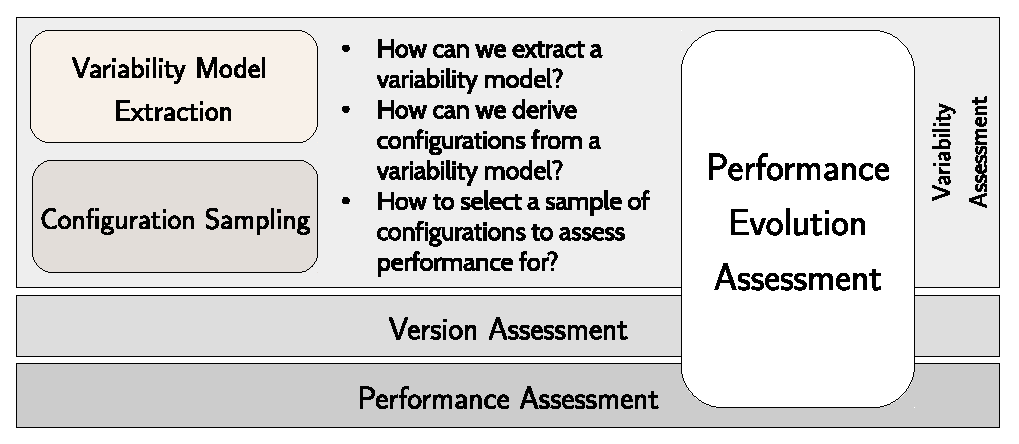
\includegraphics[width=0.90\textwidth]{images/process_varassesment.eps}
	\caption{Methodological roadmap: questions to address during variability
	assessment.}
	\label{fig:roadmap_1}
\end{figure}
 
This chapter describes the first aspect in our methodology, the assessment of
variability. As illustrated in Figure \ref{fig:roadmap_1}, this first tier of
our methodology embraces two main tasks, first, the synthesis (or extraction) of a variability model for a configurable software system, and second, strategies to select
meaningful sample sets of configurations to assess performance for. In
section~\ref{sec:untangling} we review the synthesis of variability models as
well as corresponding analyses of systems’ variability; in
section~\ref{sec:configuration_gen} we describe means to generate configurations from variability models, and finally,
section~\ref{sec:configuration_sam} discusses different strategies for selecting
sample sets of configurations.

\section{Untangling Variability}\label{sec:untangling}
Before presenting strategies to synthesize variability models in
the next section, we first recap a number of techniques to untangle configurable
software composed from variable and invariant code. In the context of our
methodology, these techniques are useful means to make variable code segments
visible, and to understand how variability influences the overall resulting
variants of a software systems.

The idea of designing and developing configurable software systems is driven by
the separation of different concerns, expressed as features of a software
system. A configurable software system is either assembled at compile-time with
respect to its configuration, or tailored to a configuration at
load-time. Both ways of implementing the variability exist in practice. Research
has also proposed a variety of variant-generating implementation techniques for
compile-time variability, ranging from simple preprocessor directives to
features as separate modules \citep{kastner_model_2009}.  A complete survey of means to implement
configurable software systems would likely exceed the scope of this section, yet we intend to discuss in this
section which information regarding variability is required or useful to our
methodology, and how it can be obtained.

\subsection{Family-based Analyses}
As the number of variants for configurable software systems is usually
infeasible, naive analyses of configurable systems are not trivial. Any static
analysis can only assess one variant at a time, as well as dynamic analyses,
which can follow only one execution path. 
In contrast to that, recently,
extended analysis techniques, which are aware of variability of the systems
studied, have emerged \citep{thum_classification_2014}. In particular, these
\emph{family-based} analyses avoid redundant computation, such as visiting a
code section multiple times, and exploit artifacts shared by multiple variants
\citep{thum_classification_2014}. Besides more efficient analysis, family-based
methods incorporate knowledge about valid feature combinations
\citep{thum_classification_2014} and, therefore, connect analysis results with
a context, such as feature combinations, for which the findings hold.
Family-based methods have been widely used across various domains and can
provide useful information when assessing configurable software systems.

\paragraph{Variability-aware Parsing.} \cite{kastner_variability-aware_2011}
have proposed the framework \emph{TypeChef} to enable the construction of
variability-aware parsers. A variability-aware parser, like ordinary parsers,
systematically explores a program to return an abstract representation of the
parsed program. This parse tree, or abstract syntax tree,
is the basis for compilers to translate a program, or for further static
analyses, such as type checking. For a code base with variability expressed by
preprocessor annotations, which are evaluated prior to compilation, a
variability-aware parser, however, is able to derive a parse tree considering
all variants in a single run. A parse tree usually consists of nodes
representing syntactical features of the parsed program. The parse tree
returned by a variability-aware parser, moreover, comprehends variable segments
of a program and will include them with respect to their presence conditions.
For instance, a class may contain a function \textit{sort()}, for which two
different implementations exist. While there might be numerous variants, the parse tree
of the class will contain a node with two children, one for each
implementation; higher numbers of alternative implementations are expressed by
nesting further nodes. In that way, variable and invariant program segments
can be separated.

While the approach of \cite{kastner_variability-aware_2011} handles
undisciplined usage of preprocessor directives, such as splitting function parameter lists, variable types, or
expressions, \cite{medeiros_discipline_2017} have proposed an approach to avoid and
conservatively refactor those cases. The authors propose a catalog of
refactoring templates, which describe transformations from undisciplined usage
of preprocessor annotations to disciplined ones. With respect to
variability-aware parsing, disciplined usage is conceived as using preprocessor
annotations only to segment statements, but not to segment a single syntactical
unit, such as expressions \citep{medeiros_discipline_2017}.

In the context of our methodology, the parse tree resulting from
variability-aware parsing can be used as a basis for further analyses. Since
the parse tree provides a machine-readable decomposition of variable and
invariant code segments along with presence conditions, for instance, it has
been used to derive constraints among features
\citep{nadi_mining_2014,nadi_where_2015} as we will see in the next subsection.


\paragraph{Staged Variability.} Besides variability-aware parsing,
\cite{nguyen_building_2014} have applied symbolic execution
\citep{king_symbolic_1976,darringer_applications_1978} to unwind variability for
PHP Web applications. Web applications are staged, i.e., even though they can be
configured at load-time, the application is as well variable with respect to
input received at run-time. For instance, consider \emph{WordPress}, a popular
content management system (CMS) implemented in PHP, which can be extended with a number
of plug-ins. However, the content of a website presented to the user also depends
on information retrieved from a database, and user input. Consequently, a
dynamic PHP Web application is staged in a sense that it generates configurable
HTML templates which are rendered at run-time. The authors utilize a symbolic
execution engine to explore all possible execution paths. Each user input or
database query is considered a symbolic value which is propagated through each script.
By keeping track of the (partially symbolic) HTML output and organizing it in a
DOM-like structure, their approach approximates the HTML output, which
subsequently can be tested, for instance for validity
\citep{nguyen_auto-locating_2011}.
Similarly, \cite{lillack_tracking_2014} have applied taint-analysis to configurable software
systems to track the influence of configuration options read at load-time.
Their static analysis approach taints every value resulting from reading a
configuration parameter as well as every value resulting from a computation
that involves previously tainted values. That way, lines of code that are
possibly depending on configuration options are detected.

In the context of our methodology, addressing staged variability with techniques
such as symbolic execution is required to assess performance for Web
applications. Both the code executed at server-side as well as the dynamically
generated HTML are interdependent parts of the Web application. Any suitable and
elaborate performance measurement setup for Web applications must incorporate
both stages.

\paragraph{Build System Variability.} Apart from
configuring software systems using preprocessor annotations, the assembling of
a configurable software system can as well be orchestrated by its underlying
build system. While preprocessor annotations virtually separate code fragments
of different features, for instance, build systems can physically exclude files
from compilation. This implementation of variability enabled by build systems,
in particular of Makefiles, has been subject to a couple of analysis approaches.
\cite{tamrawi_build_2012} have proposed \emph{Symake}, a symbolic execution
engine to evaluate Makefiles.
On top of \emph{Symake}, \cite{zhou_extracting_2015} utilize symbolic execution
to analyze Makefiles and derive file presence conditions, stating under which feature
selection a file is included or excluded from compilation. The work of
\cite{al-kofahi_escaping_2016} addresses a more advanced build system, \emph{GNU
Automake}. \emph{Automake} describes a staged build process, where a Makefile
can be specified on a higher level, and is subsequently compiled to an actual Makefile. The
authors’ aim to provide a variability-aware representation of all possible
Makefiles to enable further analyses of the build process.

In the context of out methodology, the symbolic evaluation of a software
system’s build process follows an intention similar to the one of
variability-aware parsing. Not only could further analysis tools be build upon
a symbolic evaluation engine, but also does symbolic evaluation in this context
untangle the variability accommodated in the build process. The file presence
conditions extracted by \cite{zhou_extracting_2015}
and \cite{al-kofahi_escaping_2016} are a strong basis for further constraint
extraction, and therefore variability model assessment.\\

In the context of our methodology, the mentioned family-based analyses serve two
fundamental purposes. \emph{First}, family-based analyses can help to obtain an
overview of what, or how much code in a configurable software system is variable
as well as to which extent.
For instance, if most extracted presence conditions contain only very few
features, higher-order feature interactions are unlikely. \emph{Second},
family-based analyses provide a feasible means to untangle variability and, as we will see in the
next section, are the basis for some elaborate techniques to extract
variability models \citep{nadi_mining_2014,nadi_where_2015}. In conclusion,
these analyses are not essential to extract variability models, yet are useful tools to use in
addition to the strategies mentioned in the next section.

\subsection{Variability Model Synthesis} \label{sec:feature_model_synthesis} 
A variability model as an abstraction of functionality of a software system is
required, or at least of great interest, in many contexts. Not every
configurable system provides an explicit representation of its variability
model. The reasons for inexplicit or absent configuration specification are
manifold. They can range from poor or inconsistent documentation
\citep{rabkin_static_2011} to overly complex configurability
\citep{xu_hey_2015}, or configuration constraints originated in different layers of a software system,
such as build constraints or compiler constraints
\citep{nadi_mining_2014,nadi_where_2015}.
The following paragraphs review different \emph{strategies to synthesize
variability models} from different types of artifacts. A classification of
strategies, along with corresponding literature is illustrated in Figure~\ref{fig:varsynth_overview}
The first category comprises extraction based on Natural Language Processing (NLP) utilize
similarities between textual representations of different variants to derive
common features \citep{alves_exploratory_2008,bakar_feature_2015}. The
approaches in the second category are heuristics based on static analyses, whereby configuration option names \citep{rabkin_static_2011} are
extracted, or constraints are derived from assessing the software’s build
process \citep{nadi_mining_2014,nadi_where_2015}. The last category comprises
techniques which conceive variability model as an optimization problem. For a set of given and
valid configurations, genetic algorithms are used to approximate an optimal
feature model representing constraints among features 
\citep{lopez-herrejon_reverse_2012,lopez-herrejon_assessment_2015,linsbauer_feature_2014}.

\begin{figure}[h!]
\centering
\begin{tikzpicture}[sibling distance=13em,
  every node/.style = {rounded corners,
    draw, align=center,
    top color=white, bottom color=blue!20},thick,scale=0.95, every
    node/.style={scale=0.95}]
  \node {\sffamily\bfseries Variability Model Synthesis}
    child { node [align=left] {{\begin{tabular}{c}{\sffamily NLP-based
    Extraction} \\
    \citep{alves_exploratory_2008} \\ \citep{bakar_feature_2015}
    \end{tabular}}}} 
    child { node [align=left] {\begin{tabular}{c} {\sffamily Static
    Analyses}\end{tabular}} child { node [align=left] {\begin{tabular}{c}
    {\sffamily Feature Extraction} \\
    	\citep{rabkin_static_2011}
    	\end{tabular}}} 
    	child { node [align=left] {\begin{tabular}{c} {\sffamily Constraint
    	Extraction}
    	\\
    	\citep{nadi_mining_2014,nadi_where_2015}
    	\end{tabular}}} }
    child { node [align=left] {\begin{tabular}{c} {\sffamily Feature-Model
    Approximation} \\
    \citep{lopez-herrejon_reverse_2012,lopez-herrejon_assessment_2015} \\
    \citep{linsbauer_feature_2014}\end{tabular}}};
\end{tikzpicture}
\caption{Overview of our literature survey on
variability model synthesis.}\label{fig:varsynth_overview}
\end{figure}

\paragraph{NLP-based Extraction.} As feature diagrams group and organize
features (representing functionality), synthesizing a variability model has shown to be applicable to extract features
and constraints from natural language artifacts. For instance, by comparing
product specifications for an existing market domain, variability models can
provide a detailed feature summary \citep{alves_exploratory_2008}.

The basic idea is to identify commonalities and differences in natural language
documents, such as product descriptions, requirements, or documentations, by
using natural language processing (NLP) techniques \citep{bakar_feature_2015}. A
widely employed technique is to conceive a text as a vector in a vector space model, where each word or
token represents a dimension. From the tokenized text, irrelevant stop words
are removed, and all remaining words are reduced to their original word stems.
The importance of all remaining tokens is (usually) weighed by its tf-idf
value, an established technique in information retrieval. That is, each text
(corresponding to a variant or configuration) is represented as a vector of
tf-idf values in the aforementioned vector space model. 
Based on these representations, text instances are clustered to identify
commonalities and differences, for instance in terms of shared words.
Subsequently, the clustering information can be used to extract features or entire feature
models \citep{alves_exploratory_2008,bakar_feature_2015}.

\paragraph{Feature Extraction.} \cite{rabkin_static_2011} proposed a static, yet
heuristic approach to extract configuration options along with respective types and domains. Their approach
exploits the usage of configuration APIs and works
in two stages. It commences with extracting all code sections where
configuration options are parsed. Next, configuration names can be
recovered as they are either already specified at compile-time or can be
reconstructed using string analysis yielding respective regular expressions.
Moreover, the authors employ a number of heuristics to infer the type of parsed
options as well as respective domains. \emph{First}, the return type of the
parsing method is likely to indicate the type of the configuration option read.
\emph{Second}, if a string value is read initially, the library method it is
passed to can reveal valuable information about the actual type. For instance, a method
\texttt{parseInteger} is likely to parse an integer value. \emph{Third},
whenever a parsed configuration option is compared against a constant, expression, or value
of an enum class, these might indicate valid values or at least corner cases of
the configuration option domain. The extraction method by
\cite{rabkin_static_2011} is precise, but limited, for instance, when an
option leaves the scope of the source code and is passed to a database.
Nonetheless, for the systems studied, the authors were able to recover
configuration options that were not documented, only used for debugging or even not used at
all.

\paragraph{Constraint Extraction.} 
A more comprehensive investigation of configuration
constraints and their origin is provided by
\cite{nadi_mining_2014,nadi_where_2015}. They use variability-aware parsing to
infer constraints by evaluating Makefiles and  analyzing preprocessor
directives. Inferred constraints result from violations of two assumed rules,
where (a) every valid configuration must not contain build-time errors and (b)
every valid configuration should result in a lexically different program.
While the
first rule aims at inferring constraints that prevent build-time errors, the
second one is intended to detect features without any effect, at least as part
of some configurations. Their analysis has shown a high accuracy
in recovering constraints with 93\,\% for constraints inferred by the first rule
and 77\,\% for second one respectively. However, their approach
recovered only 28\,\% of all constraints present in the software system.
Further qualitative investigation, including developer interviews, lead to
the conclusion that most of existing constraints stem from domain knowledge
\citep{nadi_where_2015}.

\paragraph{Feature-Model Approximation.}
A different strategy to recover variability models, instead of analyzing the
software artifacts, is to approximate a model. Given a selection of valid
feature selections, a variability model best describing the configurations can
be approximated, or learned. \cite{lopez-herrejon_assessment_2015} have surveyed
different search-based strategies to synthesize feature models of which we
present two categories. Evolutionary algorithms have been applied to reverse
engineer feature models from configuration samples
\citep{lopez-herrejon_reverse_2012,linsbauer_feature_2014}. A population of
feature models is generated and each instance is evaluated by a fitness
function, measuring how well it fits the given sample set of configurations.
Subsequently, a new generation is obtained by applying crossover and mutation
operators to the previous generation, whereby only the fittest instances remain.
This process of evolution is repeated multiple times until a desired threshold fitness is reached for a feature model instance.
\cite{lopez-herrejon_reverse_2012} identify a trade-off between the accuracy of
recovered feature models and the number of generations employed by evolutionary
algorithms. Besides promising results, the authors stress the importance of
effective and scalable fitness functions as well as meaningful samples to learn
the feature model from.
Contrary to evolutionary algorithms,
\cite{haslinger_reverse_2011,haslinger_extracting_2013} have proposed an ad-hoc
algorithm to reverse engineer feature models. The algorithm recovers
the feature model layer by layer via extracting all child
features for a given parent feature recursively. The algorithm does not consider
cross-tree constraints.
Besides promising results for basic feature models, the authors advocate the
incorporation of human domain-knowledge in the synthesis of feature models.
 
\paragraph{Feature-Hierarchy Recovery.} \label{sec:feature_hierarchy}
Besides recovering features and their respective constraints, to reverse
engineer a feature model, one further step is required when the outcome should
be human readable in a feature diagram. The recovered knowledge can be
organized in a tree-like hierarchy with feature groups specified and cross-tree
constraints explicitly stated to derive a valid feature diagram
\citep{kang_feature-oriented_1990}.
While several approaches for recovering the feature-model hierarchy have been
proposed, we are primarily interested in finding a hierarchy for knowledge
obtained from source code. In the remainder of this
subsection, we will focus on organizing features and constraints extracted from
source code.

Given an extracted set of features along with corresponding descriptions and
recovered constraints among the features, \cite{she_reverse_2011} propose a
semi-automated and interactive approach to synthesize a feature hierarchy.
Their approach comprises three steps. \emph{First}, an overall feature hierarchy
based on feature implications is specified. \emph{Second}, potential feature
groups are detected and manually selected. \emph{Finally}, the feature diagram
is extended with remaining CTCs. 
The approach by \cite{she_reverse_2011} provides a practical algorithm to synthesize a
feature diagram, yet has some limitations we need to consider. \emph{First}, the
approach is not able to detect or-groups as defined in Sec. \ref{sec:variability_modeling}.
\emph{Second}, the approach does introduce a root feature. \emph{Finally}, the
approach does not distinguish between mandatory and optional features. Implicitly, all features
that do not have a parent feature are optional and all features that have a
parent feature are by default mandatory. \cite{she_reverse_2011} evaluated the
algorithm with both complete and incomplete variability knowledge (feature
names, descriptions and constraints). While the algorithm has shown to be
practical, detecting features whose parent was the root-feature was difficult
since, due to the transitive property of implication, it is implied by each
feature of the feature model.\\

%\begin{enumerate}
%  \item The algorithm commences with finding a single parent for each
%  feature and, thus, specifying a tree-like feature hierarchy. Based on the
%  given constraints, a directed acyclic graph (DAG) representing implication
%  relationships among features, a so-called \emph{implication graph}, is
%  constructed.
%  Every vertex in the implication graph represents a feature  and edges are
%  inserted for each pair of features $(u, v)$, where  $u \implies v$ holds with
%  % respect to the given constraints.
%   
%  In addition to the implication graph, the algorithm for each feature computes
%  two rankings of features that are likely to be the respective parent feature.
%  The two rankings both employ the feature descriptions. Feature descriptions
%  are compared for similarity using a similarity metric. For two features $p$
%  and $s$, the similarity is defined as the weighted sum of the inverse
%  % document frequencies $idf(w)$ for the words that both descriptions of
% features $p$%  and $s$ share.

%  The $idf$-ranking for a word $w$ is the logarithm of the number of features
%  divided by the number of features whose description contains $w$. Each $idf$
%  value is weighted with the frequency of $w$ in the description of
%  feature $p$.
  
%  The first ranking, called Ranked-Implied-Features (RIF), for each feature $f$
%  ranks all features by their similarity to $f$ in an descending order, but
%  prioritizes those features that are implied according to the previously
%  computed implication graph. The second ranking, called Ranked-All-Features
%  (RAF) is similar to RIF, yet less strict since implied features are not
%  prioritized. Given these rankings, a user for each feature selects a suitable
%  parent feature from the RIF or RAF ranking. The idea behind providing two
%  separate rankings, according to \cite{she_reverse_2011} is that the given
%  extracted constraints can be incomplete and, thus, not all relevant
%  implications are contained in the implication graph.

%  \item After the feature hierarchy is specified, another auxiliary graph, a
%  mutex graph, similar to the implication graph, is constructed. The
%  % \emph{mutex graph} is an undirected graph with features as vertices and
%  % edges between two
%  features $u$ and $v$, if $u \implies \neg{v}$ and $v \implies \neg{u}$ hold
%  with respect to the given constraints. 
%  That is, all adjacent features are mutually exclusive. Based on
%  this mutex graph, all maximal cliques (subsets of vertices that all are
%  connected with each other) among the vertices with the same parent are
%  computed. All features within such a clique are mutually exclusive and share
%  the same parent and represent mutex- or alternative-groups.
  % \cite{she_reverse_2011} introduce an additional constraint to extract xor-groups that require one of the groups’
%  features to be selected if the parent is selected. This distinction is in
%  line with the initial description of feature diagrams by
  % \cite{kang_feature-oriented_1990}, but not all descriptions of feature diagrams follow this distinction between
%  mutex- and xor-groups and just use the term alternative-group discussed in 
%  Sec. \ref{sec:variability_modeling}. %2.1
  
 % \item CTCs for the feature diagram are extracted from
 % the given configuration constraints. Since CTCs are constraints that could
 % not be represented by the feature hierarchy (implication) or
 % alternative-groups (exclusion), the derivation of CTCs follows this idea. The
%  set of cross-tree implications is derived by removing all edges that are part
%  of the feature hierarchy from the initially constructed implication graph.
%  The set of cross-tree exclusions is derived similarly from the mutex
%  graph by removing all edges among vertices of all mutex-groups. To make the
%  feature model sound, the given configuration constraints, reduced to those
%  clauses that are not already entailed by the diagram, can be added as an
%  additional CTC formula to the feature diagram \citep{she_reverse_2011}.
%\end{enumerate}

Although the approaches mentioned in the paragraphs above, excluding the
feature-hierarchy recovery, in principal address the same problem, they are
isolated solutions to the problem of variability assessment, and their
applicability is depending on a number of cross-cutting boundary conditions.
\emph{First}, for the overall problem of variability model synthesis we can
identify two different contexts for which different techniques apply. The NLP-based
techniques summarized by \cite{alves_exploratory_2008} and \cite{bakar_feature_2015} address
the extraction of features in the context of requirements engineering, for instance by comparing different
software products in the same market domain. However, the remaining techniques
intend to extract features for a given single software system.
\emph{Second}, for variability assessment there exist two different principal
analysis approaches. While the techniques proposed by \cite{nadi_mining_2014,nadi_where_2015}
and \cite{rabkin_static_2011} approach a configurable software system as a monolithic system,
both the family of NLP-based techniques and the approximative techniques
\cite{lopez-herrejon_reverse_2012,lopez-herrejon_assessment_2015,linsbauer_feature_2014}
explicitly require a set of variants or configurations, respectively.
\emph{Third}, the techniques differ in the type of variability they are able to
extract variability models for. While Nadi’s approach only works for build-time
variability, the work of \cite{rabkin_static_2011} will only work for configurations read at
load-time. Moreover, the remaining techniques do not consider the different types of
variability at all.

In conclusion, it becomes clear that there is no single textbook solution to
the problem of variability model assessment as this problem may arise in
different contexts be approached from different perspectives, or be emergent
for different types of variability.

\subsection{Methodological Strategies}
The last two subsections reviewed a number of family-based analyses for
configurable software systems as well as approaches proposed to partially
extract variability models from a system’s code base. The latter approaches
presented, however, are rather isolated solutions due to non-generic
assumptions, such as the use of configuration APIs \citep{rabkin_static_2011},
or build-time variability \citep{nadi_where_2015}. At best, these approaches
complement each other, or are an appropriate choice under certain
circumstances, still requiring further manual assessment. The following
integrates the previously discussed work and proposes methodological strategies
to synthesize variability models for different scenarios, or use cases.

For the recovery of variability models, we propose three scenarios. Clearly,
this is not an exhaustive list, but covers the majority of use cases based on
our literature review. The scenarios should provide a practical context to the
previously mentioned techniques. The three scenarios are outlined in Table
\ref{tab:synthesis}; we derive our scenarios based on three criteria.
\emph{First}, we ask whether, and if so, to what extent configurability for a
software system is documented. \emph{Second}, we ask whether the software
system provides sample configurations, such as configuration presets, or
whether it ships as different variants, such as different Windows flavors.
\emph{Last}, we ask whether a variability model is explicitly contained in the
software, and whether it is visible to practitioners, such as the \emph{Kconfig}
system for the Linux kernel. For each scenario, in Table \ref{tab:synthesis},
satisfaction of either criterion is marked. In addition, we mark criteria as
\emph{satisfied optionally}, if we assume them to be satisfied, but they are
not necessarily relevant for the choice of strategy.

\begin{table} 
	\centering
	\begin{tabular}{lccc}%
	\toprule
	\textbf{Criterion} & \textbf{Scenario A} & \textbf{Scenario B} &
	\textbf{Scenario C}
	\\
	\midrule
	\mbox{Configurability documentated?} & $\surd$ & $(\surd)$ & $(\surd)$ \\
	\mbox{Configurations provided?} & $\times$ & $\surd$ & $(\surd)$ \\
	\mbox{Variability model provided?} & $\times$ & $\times$ & $\surd$ \\
	\bottomrule
	\end{tabular}\\
	\vspace{1mm}
	{\footnotesize $\surd = \text{Criterion satisfied}$, $(\surd) =
	\text{Criterion satisfied optionally}$, $\times = \text{Criterion not
	satisfied}$}
	\caption{Distinction of three scenarios for variability model synthesis. }
	\label{tab:synthesis}
\end{table}

Apparently, the latter scenario C in Table \ref{tab:synthesis} requires only
little to no assessment of the application's variability since the variability
model is already available.


\begin{sidewaystable}
  \thisfloatpagestyle{empty}  
  \centering
  
  \begin{tabular}{L{0.22\textwidth} L{0.48\textwidth} L{0.3\textwidth}}
  
  	\toprule 
    {\bf Question} & {\bf What approach or technique to use?} & {\bf
    Information Gain} \\
    \midrule
    
    {How is variability implemented?\linebreak
	{\footnotesize\it Variability can be accommodated at build- or 	load-time.}} & 
	
	{\smaller\begin{compactitem}
	  \item Manual review of the documentation with respect to what configuration
	  mechanism is used, such as run-time parameters or preprocessor annotations.
	  \item Family-based variability analyses help understand what parts of the
	  software are variable and how they are enabled, or made accessible.	  
	\end{compactitem}} & 
	
	{Knowledge of whether the software must be compiled for each configuration, or only for each version.}\\
	
	\midrule
	
	{How can the software be configured?\linebreak
	{\footnotesize\it Variability can be implemented in various ways.}} &
	
	{\smaller\begin{compactitem}
	  \item Manual review of the documentation with respect to how configurations
	  are actually encoded to be machine-readable. Look out for standard or example
	  configurations.
	 \end{compactitem}}
	  &
	
	{Knowledge about how a configuration can be translated to a machine-readable
	format required by the software, such as argument lists or preprocessor annotations.}\\
	
	\midrule
	
	{Which configuration options exist, including types and domains?\linebreak
	{\footnotesize\it Configuration options can be binary or numeric options.}} & 
	
	{\smaller\begin{compactitem}
	  \item List all configuration options mentioned in the documentation. Unless
	  not provided, consider standard or sample configurations or option names to
	  infer a type, and valid values and corresponding domains.
	\end{compactitem}} &
	
	{Knowledge about what configuration options exist, whether they are binary or
	numeric options, and what valid values can be assigned to them.}\\
	
	\midrule
	
	{Which dependencies or exist between and among configuration options?} & 
	
	{\smaller\begin{compactitem}
	  \item Manual review of the configuration options with respect to implied,
	  excluded, or alternative configuration options. Similarly, numeric
	  constraints may exist. 
	\end{compactitem}} &
	
	{Obtaining a (approximated) variability model, which is required to decide
	whether a configuration is valid or not.}\\
	
	\midrule
	
	{Has the feature model been changed during evolution?} & 
	
	{\smaller\begin{compactitem} 
		\item Review of release notes and changes in the documentation with respect to
		new features as well as constraints added, modified, or removed. 
		\item Manual inspection of changes over time in code sections where
		configuration options are read. 
	\end{compactitem}} & 
	
	{Knowledge about whether synthesizing different versions of the variability
	model is required.}\\
    \bottomrule
  \end{tabular}
  \caption{Questionnaire for manual variability
  assessment.}\label{tab:manual_var_assessment}
\end{sidewaystable}

For scenario B, despite documentation might be available, the
previously presented variability model approximation approaches
\citep{haslinger_reverse_2011,haslinger_extracting_2013,lopez-herrejon_reverse_2012,linsbauer_feature_2014}
can be applied, yet only binary configuration options are supported so far.
Given the existence of sample configuration or configuration presets, these
may provide additional information to answer the questions stated above. 
The remaining approaches mentioned in the previous subsections, unfortunately,
describe only isolated solutions. Given suitable circumstances, they can
nevertheless aid the extraction of variability models. The overall scheme in
synthesizing a variability model is to answer the the questions above manually,
and refer to automated tool support whenever possible.

For scenario A, when the main source of information regarding variability is
the software system's documentation, we are left with no other option than manual
assessment. To do so, we provide a questionnaire of
five main questions to be anwered in Table~\ref{tab:manual_var_assessment}.
The corners of the questionnaire cover, besides the manual synthesis of the
variability model, the questions of how variability is implemented,
configurations are encoded, and whether the variability model has changed
during evolution. Although the automated approaches discusses earlier are only
applicable for scenarios B or C, or under specific circumstances, family-based
analyses can support manual assessment.

We have seen that the extent to which automated solutions are applicable to
variability assessment depends on the degree to which variability is
documented. If the variability model is available  in a machine-readable
format, little to no further assessment is required, while, if documentation was
done manually, so variability assessment remains a task to be done manually. 
In conclusion, the questionnaire in Table~\ref{tab:manual_var_assessment} covers
most aspects required to comprehend variability for a configurable software system and can be
conceived as a guideline. Whenever applicable, additional synthesis or analysis
techniques can be taken into account.

\section{Configuration Generation}\label{sec:configuration_gen}
The next intermediate step in our methodology is the generation of
configurations from the variability model. Once obtained, we use the
variability model to derive valid feature selections. For the assessment of
quality attributes for configurable software systems, such as test case
coverage or performance, we usually assess a sample set of variants. Hence, we
require techniques to derive valid feature selections from the variability
model to select meaningful sample sets from. As there exist various forms to
express a variability model, configurations may be generated in various ways.
Variability models can, for instance, be expressed as propositional formulas,
context-free grammars (CFG) \citep{batory_feature_2005}, or constraint
satisfaction problems (CSP)
\citep{benavides_automated_2005,benavides_using_2005}. Accordingly, all configurations represent solutions to propositional formulas or CSPs, or valid words for CFGs
respectively. That is, the generation of all configurations with respect to the
variability model is equivalent to finding a solution or sentence for the
aforementioned representations of a variability model. In the following, we
review how variability models can be encoded as a CSP and describe in detail
the configuration generation using CFGs.

\subsection{Constraint Satisfaction Problem}
A constraint satisfaction problem (CSP) in the context of variability modeling
describes a set of options ranging over finite domains as well as a set of
constraints which restrict the value range of a variable
\citep{benavides_automated_2005}. For a binary option $b$, the respective domain $dom(b)$ simply is $\lbrace 0, 1\rbrace$.
For a numeric option, the respective domain $dom(n)$ is a finite set of legal
values with a minimum and a maximum value, say $\lbrace v_{min}, v_1,
v_2, \ldots, v_{max}\rbrace$.
A solution $s: O \rightarrow dom(o_1) \times dom(o_2) \times \ldots \times
dom(o_{|O|})$ to a CSP is an assignment of options $o_i \in O, i \in \mathbb{N}$
to values of their respective domain, such that all constraints are satisfied simultaneously \citep{benavides_automated_2005}.  

A solution to a CSP is found by systematically checking for different
selections of values whether all constraints are satisfied. There exists a
large number of ready-to-use SAT and CSP solvers, yet we are not covering CSP
solution here since it is beyond the scope of the thesis. For further reading, 
\citep{benavides_fama:_2007} present a tool with extensive analysis support for
various different presentations of variability models.

To encode a variability model as a CSP, \cite{benavides_automated_2005} describe
the following transformation rules:

\begin{itemize}
  \item For a parent feature $f$ and a child feature $f’$, a mandatory
  relationship is expressed as $f \Leftrightarrow f’$, and an optional relationship is
  expressed as $f’ \implies f$.
    \item  For a parent feature $f$ and child features $f_i$, where $i = 1, 2,
    \ldots n$, an or-group is expressed as $f \Leftrightarrow f_1 \lor f_2 \lor
    \ldots \lor f_n$, and an alternative-group is expressed as $$\bigwedge_{i
    = 0}^n f_i \Leftrightarrow (f \land \bigwedge_{j \in \lbrack 0, n \rbrack
    \setminus i} \neg f_j) $$.
\end{itemize}

To also consider numeric options, the domain of a numeric option $n$ can be
conceived as an alternative-group since only one value from the domain can be
selected at a time. This is often called disretization of the domain. Hence,
each value of the domain $dom(n)$ can be conceived as a binary option. If value $v \in dom(n)$ is selected, this states $n = v$,
otherwise $n \neq v$.


\subsection{Grammar Expansion}
Besides trying to find a solution for satisfiability problems, the expression of
variability models as context-free grammars (CFGs) enables the derivation of
configurations directly from a CFG by expanding it. A
first description of transformation rules, yet only for feature diagrams with
binary options, was was proposed by \cite{batory_feature_2005}. A hierarchical feature diagram
can be recovered from a set of constraints using the algorithm of
\cite{she_reverse_2011} as explained in section \ref{sec:feature_hierarchy}.
In the following, we describe
how a feature diagram with both binary and numeric features can be transformed
to a context-free grammar, and how configurations can be derived subsequently.

\begin{definition}[Context-free Grammar]\label{def:cfg}
A context-free grammar is a tuple $G = (N, T, S, P)$, consisting of a set of
non-terminal symbols $N$, a set of terminal symbols $T$, a start word $S \in (N
\cup T)^*$, and a set of productions $P \subseteq N \times (N \cup T)^*$. The
set $L_G$ describes the language of the grammar $G$ and comprises all valid
words $w \in L_G$ which can be derived from the start word $S \in L_G$ by
applying productions a finite number of times to it.
\end{definition}

Following the Definition~\ref{def:cfg}, to derive all configurations for a
given feature diagram, the idea is to first translate it to a context-free
grammar. In order to do so, especially with respect to handling numeric
options, we introduce an extended definition for a CFG, a configuration
generation grammar.

\begin{definition}[Configuration Generation Grammar]\label{def:cgg}
A configuration generation grammar is a context-free grammar $G = (N, T, S,
P)$ whose elements are constructed from a feature diagram as follows.

\begin{itemize}
  \item All features represent non-terminal symbols $N$, which can be divided
  into two disjoint sets, binary non-terminal symbols $F_\mathcal{B}$ and
  numeric non-terminal symbols $F_\mathcal{N}$. That is, $N = F_\mathcal{B}
  \cup F_\mathcal{N}$ and $F_\mathcal{B} \cap F_\mathcal{N} = \varnothing$.

  \item Similarly, the set of terminal symbols $T$ is consists of two different
  sets, the binary terminal symbols $T_\mathcal{B}$ and the numeric terminal
  symbols $T_\mathcal{N}$, so that $T = T_\mathcal{B} \cup T_\mathcal{N}$ and
  $T_\mathcal{B} \cap T_\mathcal{N} = \varnothing$ with
  
  \begin{equation}
  T_\mathcal{B} = \bigcup_{b\in F_\mathcal{B}} \lbrace b_0,  b_1\rbrace
  \end{equation}
  
  \begin{equation}
  T_\mathcal{N} = \bigcup_{n\in F_\mathcal{N}} ~ \bigcup_{v_i \in dom(n)}
  \lbrace n_{v_i}\rbrace.
  \end{equation}
  
  \item All productions $P$ are constructed from the hierarchy specified in the
  given feature diagram, the binary, and the numeric features. In our definition
  of a configuration grammar, each word $w$ is expressed as a subset of
  (non-)terminal symbols, i.e., $w \subseteq (N \cup T)$. A word is a terminal
  word, if and only if it does not contain any non-terminal symbol. Accordingly,
  the set of productions is $P \subseteq N \times (N \cup T)$, and a production
  $p = (u, v) \in P$ is applied to a word $w$ by removing non-terminal symbol
  $u$ from word $w$ and merging words $v$ and $w$. Hence, the new word $w'$ is
  defined as $w' = (w \setminus u) \cup v$.

  The productions $P = P_H \cup P_F$ are constructed from the following disjoint
  two sets of productions:
  
  \begin{equation}
  P_H = \lbrace (p, \lbrace c, c_1 \rbrace) | p, c \in N \land
  c \implies p\rbrace
  \end{equation}
  
  \begin{equation}
  P_F = \bigcup_{f \in (F_\mathcal{B} \cup F_\mathcal{N})} ~ \bigcup_{v \in
  dom(f)} \lbrace (f, v) \rbrace
  \end{equation}
	
  \item Finally, the start word $S \subseteq (N \cup T)$ consists the
  non-terminal representing the top-level feature in the given feature diagram.
  The set of respective configurations is described by all words which can be
  generated by a finite number of applications of productions to the start word
  $S$.
  
  \end{itemize}
\end{definition}

Based on Definition \ref{def:cgg}, we can specify an algorithm that computes the
transitive closure of the grammar by repeatedly expanding each non-terminal for
each (partial) word until a word containing non-terminal symbols is left.
In addition to deriving all configurations from a grammar, the
algorithm can also be used to derive partial configurations, such as
binary-only configurations. To do so, the numeric features need to be removed
from the set of non-terminal symbols. The only limitation of this algorithm is
that, conceptually, it requires all numeric options to be mandatory features.
This is due to the unspecified semantics of a numeric option being un- or
deselected.

In the context of our methodology, configuration generation remains an
intermediate step between the synthesis of a variability model and the
selection of a meaningful sample set of configurations. The results obtained
from applying both techniques, the encoding as a logical problem or the
translation to a context-free grammar,  to a variability model are equivalent.
However, both techniques differ in terms of cost and tool support. While the
former technique generally demands additional tool support, such as SAT or CSP
solvers, their use is well established among research tools, such as
\emph{FeatureIDE} \citep{al-hajjaji_incling:_2016} or \emph{SPLConqueror}
\citep{siegmund_predicting_2012}. Moreover, research has shown that SAT solvers
generally scale for large configurable software systems. 
In turn, the latter technique using context-free grammars can easily be implemented, yet the exhaustive expansion
of a context-free grammar is infeasible and does not scale since all valid
configurations are derived. Nonetheless, for handling smaller variability
models, context-free grammar might be a makeshift solution.
%\begin{algorithm}[H]\label{alg:expand}
% \KwData{Configuration generation grammar $G = \lbrace N, T, S, P \rbrace$, and
% cross-tree constraints $C$ of the given variability model}
% \KwResult{All configurations of the given variability model.}
% \vspace{5mm}
% words = Queue()\;
% words.enqueue($S$)\;
% \While{words is not empty}{
%  current = words.dequeue()\;
%  \If{current does violate any cross-tree constraint}{
%   continue\;
%   }
%   \For{$n \in N$}{
%   		\If{$n \in current$}{
%   			\For{$u \in \lbrace u | (n, u) \in P \rbrace$}{
%   				new = current\;
%   				new = new $\setminus~ n$\;
%   				new = new $\cup~ u$\;
%   				\eIf{$N \cup new = \varnothing$}{
%   					yield new\;
%   				}{
%   					words.enqueue(new)\;
%   				}
%   			}
%   			break\;
%   		}
%   }
% }
 
% \caption{Expansion algorithm for a configuration generation grammar.}
%\end{algorithm}\vspace{2mm}

\section{Configuration Sampling}\label{sec:configuration_sam}
When assessing emergent properties for configurable software systems, it is
infeasible to consider every possible variant. As previously stated in
section~\ref{sec:variability_modeling}, interactions between
features can emerge, and can be the root cause for configuration-related
performannce-interactions. Hence, effects on performance quality may be
identified only under specific configurations. To not exhaustively assess all
variants, a variety of strategies to select a sample set of configurations have been proposed.
Every sampling strategy in the context of configurable software system is
designed with respect to a \emph{coverage criterion} 
\citep{apel_feature-oriented_2013}. While some coverage criteria take into
account the coverage of feature interactions, such as t-wise sampling
\citep{williams_practical_1996}, others consider code coverage, such as
statement coverage sampling \citep{tartler_static_2014}.
Although configurations in our case can contain both binary and numeric options, we
distinguish sampling strategies for both categories. In the following, we
review a selection of popular sampling strategies for binary options as well as
sampling strategies for numeric options, especially in the context of
performance assessment.

\paragraph{Binary Features.}
Most sampling strategies in the context of configurable software systems
target binary features. Popular sampling strategies for sampling configurations
of binary features include, but are not limited to the following
\citep{apel_feature-oriented_2013,medeiros_comparison_2016} strategies listed in
Table \ref{tab:sampling}.

\begin{table}[h!]
	\centering
	\begin{tabular}{p{0.25\textwidth}p{0.7\textwidth}}
	\toprule
	\textbf{Strategy Name} & \textbf{Description} \\
	\midrule
	\mbox{Feature Coverage} & Configurations are selected, so
	that each feature is selected in at least one configuration
  \citep{apel_feature-oriented_2013}. An extension proposed by
  \cite{sarkar_cost-efficient_2015} for projective sampling takes into account
  feature frequencies. The frequency of a feature is the frequency of the
  feature being selected or deselected in a sample set. As a coverage
  criterion, a specified minimum feature frequency is to be reached.\\
  \midrule
  Most-enabled-disabled & Configurations are selected, so that a
  maximal and minimal number of features is enabled
  \citep{medeiros_comparison_2016}. \\
  \midrule
  One-enabled & Configurations are selected, so
  that each feature is enabled at a time \citep{siegmund_predicting_2012}. Similarly, with a
  \emph{one-disabled} strategy, configurations are chosen, so that each feature
  is deselected at a time. \\
  \midrule
  Random Sampling & Configurations are selected randomly, i.e., for a
  configuration, for each optional feature a random value out of 0 or 1 is
  assigned. \cite{guo_variability-aware_2013} have studied learning performance
  of a configurable software system from a random sample with acceptable
  accuracy. \\
  \midrule
  Statement-coverage & Configurations are
  selected, so that each variable block of code (for
  compile-time variability) is at least included in one
  variant \citep{tartler_static_2014}. This either applies to variable code
  sections via preprocessor annotations, or to entire files and compilation
  units. \\
  \midrule
  T-wise sampling & Configurations are selected, so that all
  t-tuples of all (binary) features are included in at least one configuration
  \citep{williams_practical_1996}. That is, the upper bound for the sample size
  is $\binom{|F|}{t}$ for features $F$ and $t \in \mathbb{N}$.
  \cite{siegmund_predicting_2012} extend this approach by composing
  higher-order feature tuples ($t > 2$) from already known pair-wise
  interactions. The rationale behind this heuristic is that, if pairs of
  features interact, also tuples including those pairs are likely to interact.\\
	\bottomrule
	\end{tabular}
	\caption{Selection of sampling strategies for binary features.}
	\label{tab:sampling}
\end{table}

\cite{medeiros_comparison_2016} have compared different sampling strategies,
among other things with respect to resulting sample size and fault detection
rate. \emph{Most-enabled-disabled} results in the smallest
sample size, whereas \emph{t-wise} sampling, especially for a greater $t$ yields
the largest samples. Regarding the detection of faults,
\emph{statement-coverage} performed poorly, whereas \emph{t-wise} sampled
samples, especially with a greater $t$ unveiled most faults. Note that
sampling with respect to statement coverage is not applicable in the context of
performance assessment since for performance measurements, the software system is generally conceived as a  black
box. 

\paragraph{Numeric Features.}
Similar to selecting meaningful sample sets of binary options, for numeric
options, sampling strategies are designed with respect to covering possible
interactions. Subsumed under the term \emph{design of experiments} various
sampling strategies, or experimental plans have been proposed, each assigning values
(from an option’s domain) to independent variables (numeric options, in this
case) \citep{antony_design_2014}. As the choice of an experimental plan (for
both binary and numeric options) determines the number of measurements, and therefore the cost of
assessment, not all designs might scale and be suitable for our assessments.
\cite{siegmund_performance-influence_2015} have reviewed and evaluated a number
of established experimental plans with respect to applicability in the context
of configurable software systems.
The authors exclude a number of designs due to an infeasible number of measurements, and advocate the use of
four designs, including the Plackett-Burman Design and Random Designs. Assuming
a discrete domain of values for each numeric option, the former design requires
each combination of levels for each pair of numeric options to occur equally.
The latter design is advocated not least because of an negligible number of
constraints among numeric options \citep{siegmund_performance-influence_2015}.
For further reading on more detailed descriptions of experimental designs, refer
to \cite{antony_design_2014}. 

In conclusion, finding a suitable sampling strategy remains a tasks with many
aspects to consider. Depending on whether binary, numeric, or both types of
configurations options are present, sampling strategies are selected,
respectively. To derive mixed configurations, first, samples are selected from
both binary and numeric configuration options. Second, the final sample of
mixed configurations is computed as the cross-product of binary and numeric
partial configurations. As stated by \cite{siegmund_performance-influence_2015}, the
treating binary and numeric options separately is justified since usually binary options enable
or disable functionality while numeric options merely tune functionality. In
the context of out methodology, a suitable sampling strategy might include
combining different strategies, either due to different types of configuration
options, or due to multiple coverage criteria to meet. As a guideline for
selecting a sampling strategy, especially in the context of performance
assessment, no clear recommendation can be given. However, from samples
selected via random sampling \citep{sarkar_cost-efficient_2015} and pair-wise
sampling \citep{siegmund_performance-influence_2015} have shown acceptable results in terms
of accuracy.
